\chapter{Trabalhos Relacionados}
\label{cap:relacionados}
Neste capítulo serão apresentadas duas ferramentas para o alinhamento de dados conectados. As ferramentas apresentadas a seguir foram selecionadas devido ao seu destaque na edição de 2016 do relatório publicado pela Ontology Alignment Evaluation Initiative (OAEI). Inicialmente, a OAEI avaliava apenas ferramentas de alinhamento de ontologias, dando início à avaliação de soluções para alinhar dados em 2009. Desde então, um número crescente aplicações vêm sendo submetidas.

\section{AgreementMakerLight (AML)}
Desenvolvido em parceria entre o Instituto Gulbenkian de Ciência, Universidade de Lisboa, e Universidade de Illinois. O AgreementMakerLight é uma ferramenta de alinhamento de ontologias. De acordo com \cite{fariaoaei}, o AML é uma ferramenta que se baseia inicialmente em técnicas e similaridade léxica, tendo como enfase o uso de fontes externas como background.

O AML conta com três algoritmos para alinhamento voltados a correspondência de instâncias, sendo elas o \textit{HybridStringMatcher}, \textit{ValueStringMatcher} e \textit{Value2LexiconMatcher}. A primeira utiliza diversas abordagens para gerar a similaridade, sendo elas a comparação entre frases, palavras. Além disso, essa abordagem hibrida também explora a \textit{WordNet}. O segundo utiliza o mapeamento de valor para gerar calcular a similaridade, penalizando pares nos quais anotações ou propriedades de dados não são os mesmos. Por fim, o terceiro une as duas abordagens anteriores.

Apesar do AML possuir diferentes algoritmos alinhamentos na ferramenta, todos eles trabalham apenas no nível dos dados. Consequentemente, as características das propriedades são desconsiderados ao longo do processo de correspondência.

\section{RiMOM-2016}
Baseando-se no RiMOM  \cite{li2009rimom}, \cite{zhang2016rimom} desenvolveram o RiMOM-2016, que é uma ferramenta para alinhar dados conectados. Ela implementa um número considerável de abordagens para alinhar, cuja escolha é realizada através dos metadados extraídos da ontologia. Além disso, o RiMOM-2016 utiliza um índice invertido para indexar os objetos e consequentemente gerar pares candidatos para um possível alinhamento. A geração dos pares é realizada quando dois recursos compartilham pelo menos um predicado e objeto.

\begin{figure}[!ht]
	\centering
	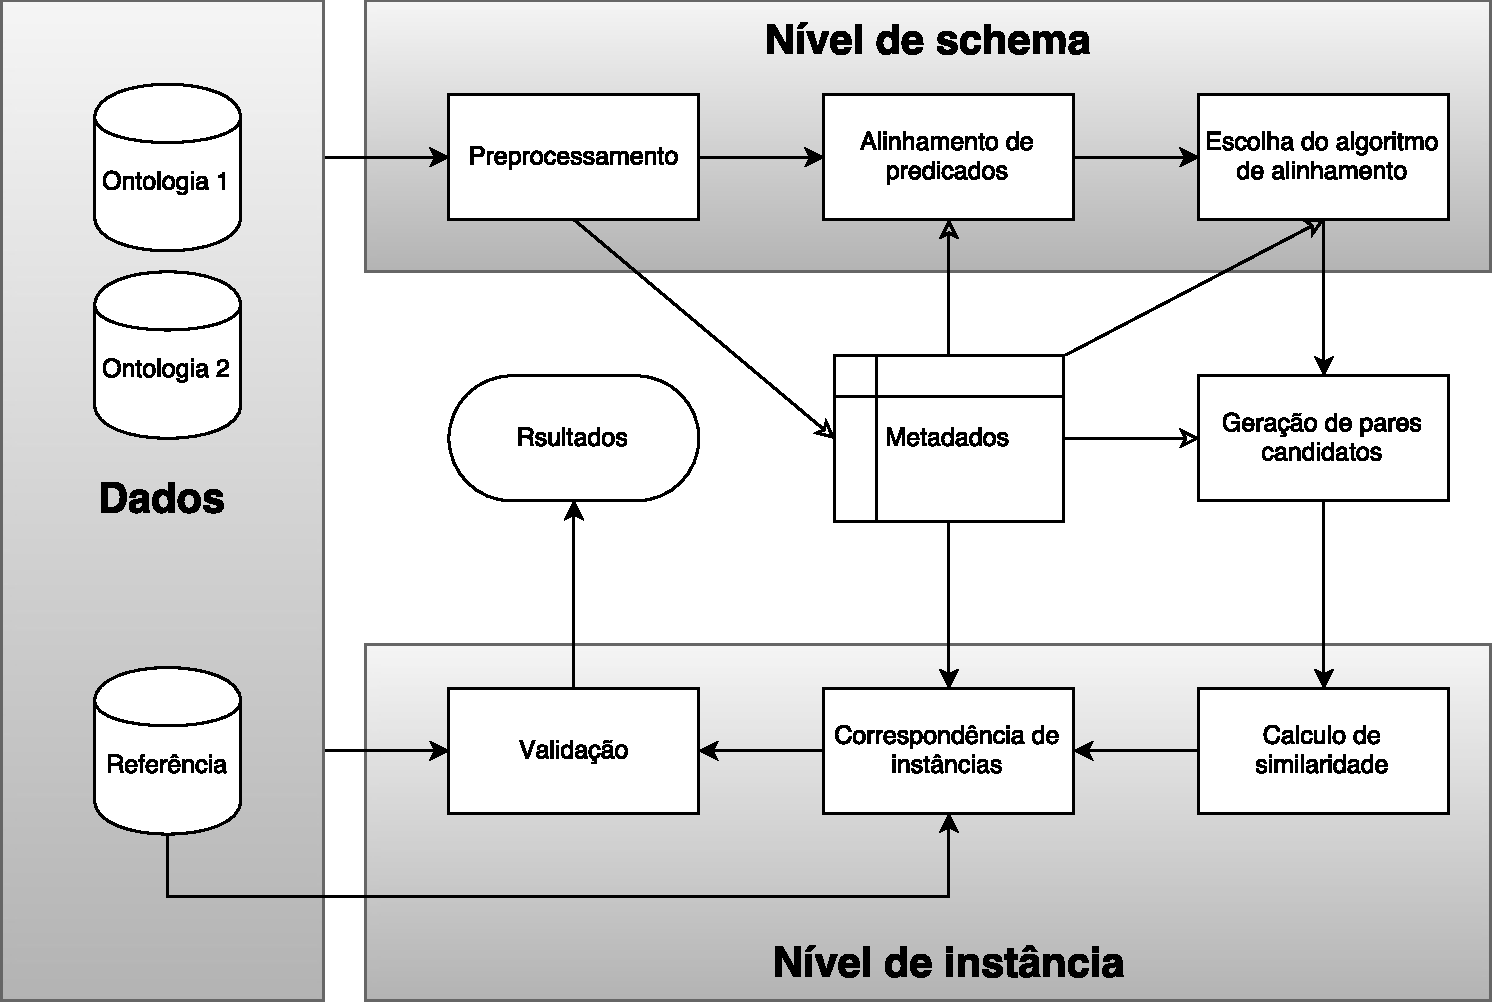
\includegraphics[width=0.8\textwidth]{./imagens/rimom_2016.pdf}
    \caption{Arquitetura do RiMOM-2016}
	\footnotesize{Fonte: adaptado de \cite{zhang2016rimom}}
	\label{fig:rimom}
\end{figure}

Por um lado, o índice invertido permite que um número menor de comparações seja realizado. Por outro lado, a etapa de construção desse índice não considera que os objetos indexados podem conter qualquer tipo de erro. Além disso, como pode ser visto na Figura \ref{fig:rimom}, o RiMOM-2016 utiliza as ontologias apenas para alinhar as propriedades e como entrada para a geração de metadados.

\section{Comparação com a proposta}

Neste capítulo, algumas das principais ferramentas existentes foram apresentadas. Estas ferramentas tem o objetivo de alinhar dados conectados através de diversas abordagens. Dentre os sistemas apresentados, nenhum deles têm o alinhamento de dados como foco principal. Além disso, as ferramentas são baseada em soluções de alinhamento de ontologias, porém a exploração no processo de alinhamento se limita à geração de metadados para auxiliar na escolha da estratégia que deve ser tomada. 

Diferentemente das ferramentas citadas, a proposta a ser apresentada utiliza a ontologia para guiar o processo de correspondência de instância. Essa abordagem permite que o usuário defina como o alinhamento deve ser realizado. A tabela \ref{tab:comparacao} sumariza e compara os trabalhos relacionados com a proposta.

\begin{table}[h]
\centering
\caption{Comparação entre os trabalhos}
\label{tab:comparacao}
\begin{tabular}{@{}ccl}
	\toprule
	Ferramenta & Suporte à ontologia & Suporte à transitividade \\ \midrule
	   AML     &      Dirigido       &  \\
	  RiMOM    &      Dirigido       &  \\
	 Proposta  &       Baseado       & X                        \\ \midrule
	           &
\end{tabular}
\end{table}
